% \renewcommand{\sd}[1]{#1}
 \newcommand{\sdOct}[1]{#1}%{{\red{#1}} 
\newcommand{\re}{\mathit{e}}

\section{\SpecLang specifications}
\label{s:semantics}

 
In this section we define {the}  \SpecLang specification language.  
We first define an underlying programming language, \LangOO (\S \ref{sub:Loo}).
We then define an assertion language, \AssertLang, which can talk about the
contents of the state, as well as about protection (\S \ref{sub:SpecO}).  Finally, we define the syntax and
semantics of  \SpecLang
specifications (\S \ref{s:holistic-guarantees}).

 


\subsection{\LangOO -- the underlying object oriented programming languages}

\subsubsection{\LangOO syntax and semantics}
\label{sub:Loo} 
%\jm[TODO: mention the type system and the restriction on external method calls]{}
%% We introduce a simple object-oriented language, \LangOO, upon 
%% which our specification language sits.
We repeat the def. of  \LangOO from oopsla. It is a {small}, imperative, sequential, 
class based, typed, object-oriented language, whose
fields are private to the class where they are defined. 
\LangOO is straightforward
{and the complete definition can be found in the appendices % of the full paper 
\cite{necessityFull}.}
 A \LangOO state $\sigma$ consists of a 
heap $\chi$, and a  {stack $\psi$ which is a sequence of frames}.
A frame $\phi$ consists of
local variable map, and a continuation, \ie a sequence of statements to be executed.
{We use  $| \sigma |$ to describe the numbers of frames in the stack of  $\sigma$, i.e. the number of nested, currently active method calls.}
 A statement may assign to variables, create new objects and push them to the heap, 
perform field reads and writes on objects,  or
 call methods on those objects. 

 
Modules are mappings from class names to class definitions. 
Execution 
takes place
 in the context of  a module $M$ and   a state $\sigma$,
 defined via unsurprising small-step semantics of the form \ \ 
   $M, \sigma \leadsto \sigma'$.
The   top frame's continuation contains the statement to be 
executed next.  


\paragraph{Applicability} 
{While our work is based on 
  a simple, imperative, typed, object oriented}
language with unforgeable addresses and private fields, we believe
 that % our approach
 it is applicable to several programming paradigms, and 
 that   unforgeability and privacy
 can be replaced 
 by lower level mechanisms such as capability machines \cite{vanproving,davis2019cheriabi}.

  \subsection{\sd{Reachable  Objects}}


\begin{definition} We define 
\begin{itemize}
\item
$\Relevant \alpha \phi \sigma $  \ \ \ \ \ \ \ iff\ \  
$\exists n\in \mathbb{N}.\exists \prg{f}_1,... \prg{f}_n.\exists \prg{x}.[ \ \interpret{\sigma}{\phi(x).\prg{f}_1.....\prg{f}_n} = \alpha  ]$.
\item
$ \LRelevant \alpha \sigma $ \ \ iff\ \  
$\exists \phi.[\ \sigma=(\phi\cdot\_, \_)$ and $\Relevant \alpha \phi \sigma\ ]$. % for some $\phi$
\item
$\GRelevant \alpha \sigma$  \ \ iff\ \  
$\exists \phi.[\ \sigma=(\_\cdot\_\phi\cdot\_, \_)$ and $\Relevant \alpha \phi \sigma\ ]$. % for some $\phi$
\end{itemize}
\end{definition}

Globally reachable objects are those that are reachable from one of the frames on the stack. The lemma below says that any object which existed in the currently heap, and becomes globally reachable at some future point is globbaly reachable now. That is, no globally unreachable object may become reachable.


\sdN{
\begin{lemma}
\label{lemma:relevant}
For all $\sigma$, $\sigma'$, for all objects $o$, and for all modules $M$:
\begin{itemize}
\item
$M, \sigma  \leadsto*   {\sigma'} \ \wedge \  \GRelevant o {\sigma'} \ \wedge \ o\in dom(\sigma) \ \ \Longrightarrow \ \  \GRelevant o {\sigma}$
\end{itemize}
\end{lemma}
}
 

\subsection{??? Semantics -- $\leadsto$}



\sd{When that statement has the form \texttt{return}, then the top frame is popped, and execution continues in the context of the calling method.
in some cases\footnote{TODO mpotivate} we are only interested in executions which may include function calls, returns from nexted function calls, 
but not return from the currently executing method.}



\sd{
\begin{definition}[??? Semantics]
\label{def:up-reduce}
For    module  $M$  and     states $\sigma$, $\sigma'$, 
we say that $\ \ \ \ \ \ \ \ \ M {\sigma}\leadstoUp {\sigma'}\ \ \ \ \ \ \ \ $ if and only if there exist 
$n\in\mathbb{N}$, and states $\sigma_0$,...$\sigma_n$, such that
\begin{enumerate}
\item
\label{up1}
$\sigma$=$\sigma_1$, and  $\sigma'$=$\sigma_n$,
\item
\label{up2}
$M, \sigma_i \leadsto \sigma_{i+1}$  \ \ \ for all $i\in [{1}..n)$,
\item
\label{up3}
{$| \sigma_1 | \leq | \sigma_i |$ \ \ \  for all $i\in [1..n]$,}
\end{enumerate} 
\end{definition}
}

\begin{figure}[htb]
\begin{tabular}{|l|l|}
\hline \\
\resizebox{6.5cm}{!}{
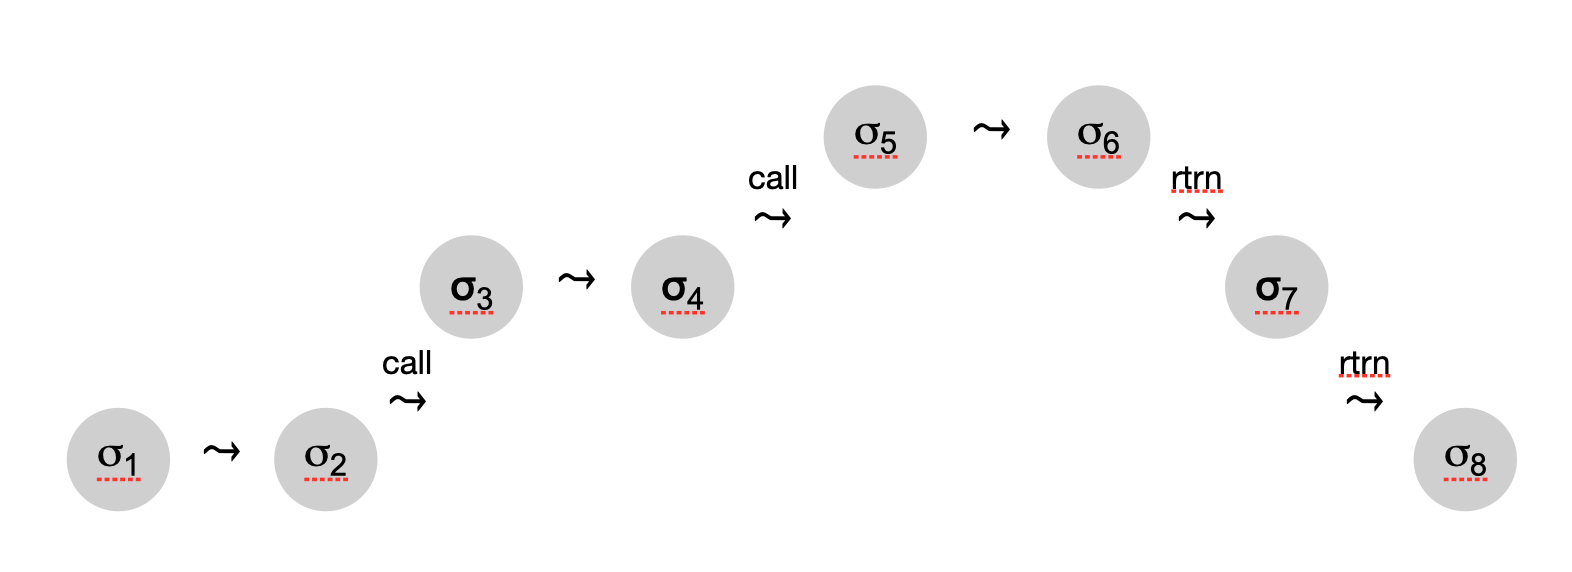
\includegraphics[width=\linewidth]{diagrams/up1.png}
} 
&
\resizebox{6.5cm}{!}{
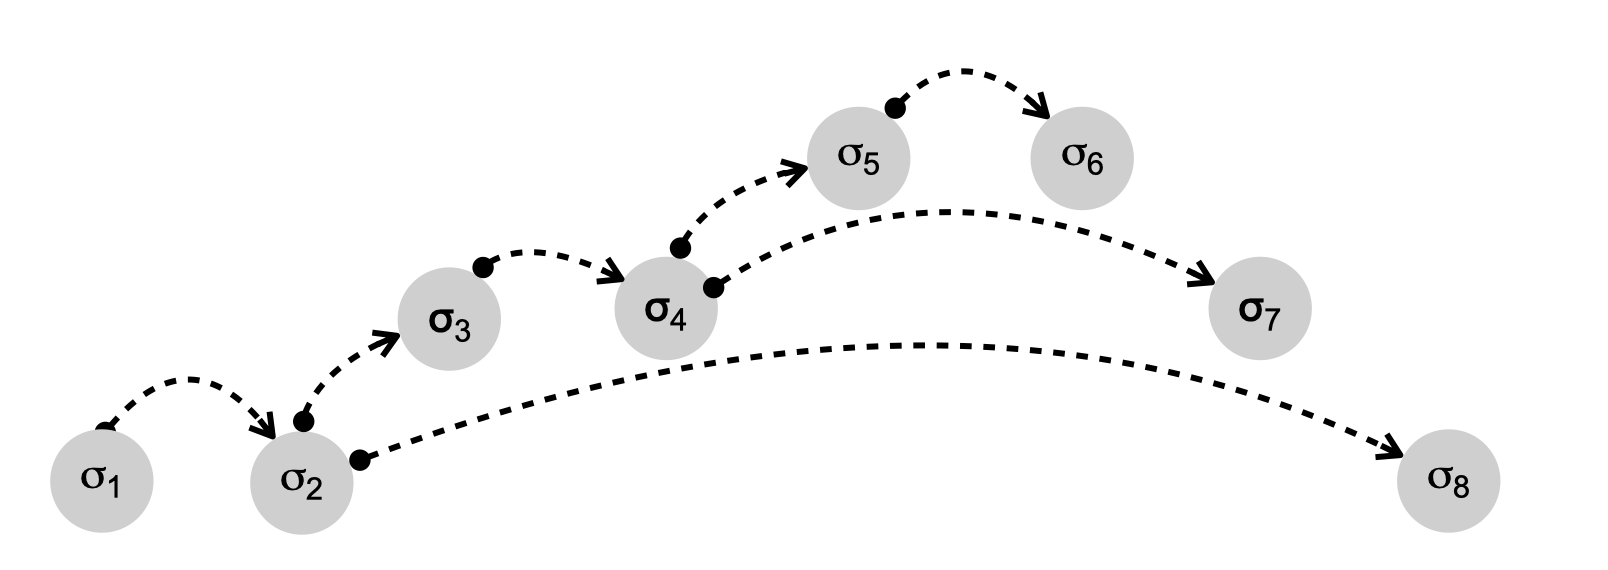
\includegraphics[width=\linewidth]{diagrams/up2.png}
}
\\
\hline
\\
$\exec{M}{{\sigma_1}} {{\sigma_2}}
 \leadsto {{\sigma_3}}  \leadsto {{\sigma_4}}
\leadsto {{\sigma_5}} $
&
${M},{{\sigma_1}} \leadstoUp {{\sigma_2}}
 \leadstoUp  {{\sigma_3}}  \leadstoUp  \leadstoUp  {{\sigma_4}}   \leadstoUp  {{\sigma_4}}   \leadstoUp     {{\sigma_6}}$
\\
$\exec{{M_{ext}} \circ {M}}{{\sigma_5}} {{\sigma_6}}
\leadsto{ {\sigma_7}}
\leadsto {{\sigma_8}}$ &
${M},{{\sigma_4}} \leadstoUp {{\sigma_7}}$
\\
& 
${M},{{\sigma_2}} \leadstoUp {{\sigma_8}}$
\\
\hline
\end{tabular}
   \caption{Illustrating ???-$\leadstoUp$  Semantics
     (Def. \ref{def:pair-reduce}) %
    }
   \label{fig:UpSemantics}
 \end{figure}


 \subsubsection{Observable States Semantics}

As discussed in \S \ref{s:approach}, 
{open world specifications need to be able to provide}
guarantees which hold
during execution of an internal, 
known, trusted module $M$ when linked together with any
unknown, untrusted, module $M_{ext}$. These guarantees need only hold 
when the external module is executing; we are not concerned if they are
temporarily broken by the internal module. Therefore, we are only interested in states where the
executing object (\prg{this}) is an external object. 
To express our focus on external states, we define the  \emph{external states semantics}, of the form 
$\reduction{M_{ext}}{M}{\sigma}{\sigma'}$, where $M_{ext}$ is the external
module, and $M$ is the internal module, and where we
collapse all internal steps into one single step.

 

\sd{
\begin{definition}[{Observable} States Semantics]
\label{def:pair-reduce}
For    modules $M$,  $M_{ext}$, and     states $\sigma$, $\sigma'$, 
we say that $\ \ \ \ \ \ \ \ \reduction{M_{ext}}{M}{\sigma}{\sigma'}\ \ \ \ \ \ \ \ $ if and only if there exist 
$n\in\mathbb{N}$, and states $\sigma_0$,...$\sigma_n$, such that
\begin{enumerate}
%\item
% \label{vis1}
% $\sigma$=$\sigma_1$, and  $\sigma'$=$\sigma_n$,
\item
\label{vis2}
%$M_{ext} \circ M, \sigma_i \leadsto  \sigma_{i+1}$  \ \ \ for all $i\in [{1}..n)$,
$M_{ext} \circ M, \sigma  \leadstoUp  \sigma'$  
\item
%\label{vis3}
%{$| \sigma_1 | \leq | \sigma_i |$ \ \ \  for all $i\in [1..n]$,}
% \item
\label{vis4}
$\class {\prg{this}}{\sigma}, \class {\prg{this}} {\sigma'}\!\in\! M_{ext}$, %\ \ \ and \ \ \
%\item
%$\class {\prg{this}} {\sigma_i}\!\in\! M$\ \ \ for all $i\!\in\! (1..n)$.
\end{enumerate} 
\end{definition}
}
{ Thus, we collapse into one step a sequence of $\leadsto$ steps (requirements \ref{vis1}  and \ref{vis2}), which may include function calls and returns but
 not returns from the method currently executing in $\sigma_1$ (requirement  \ref{vis3}), and where the starting and end states belong to the external module (requirement  \ref{vis4}), while all intermediate states belong to the internal module (requirement  \ref{vis4}).}
\footnote{TODO: update the explanations}

\footnote{{TODO: chase all references to "external states semantics".}}

Note that the   function $\class{\_}{\sigma}$ is overloaded:
when  applied to a variable, 
$\class{x}{\sigma}$  looks up the variable $x$ in the top frame of $\sigma$, and returns the 
class of the corresponding object in the  heap of $\sigma$;
applied to an address, $\class{\alpha}{\sigma}$  returns
the class of   the object referred by address $\alpha$ in the heap of $\sigma$. 
 The module linking operator $\circ$, applied to two modules, $M_{ext}\circ M$, 
 combines the two modules into one module in the obvious way, provided their
domains are disjoint.
The details {can be found in the appendices\cite{necessityFull}.} %Appendix \ref{app:loo}.
\begin{figure}[htb]
\begin{tabular}{|l|l|}
\hline \\
\resizebox{6.5cm}{!}{
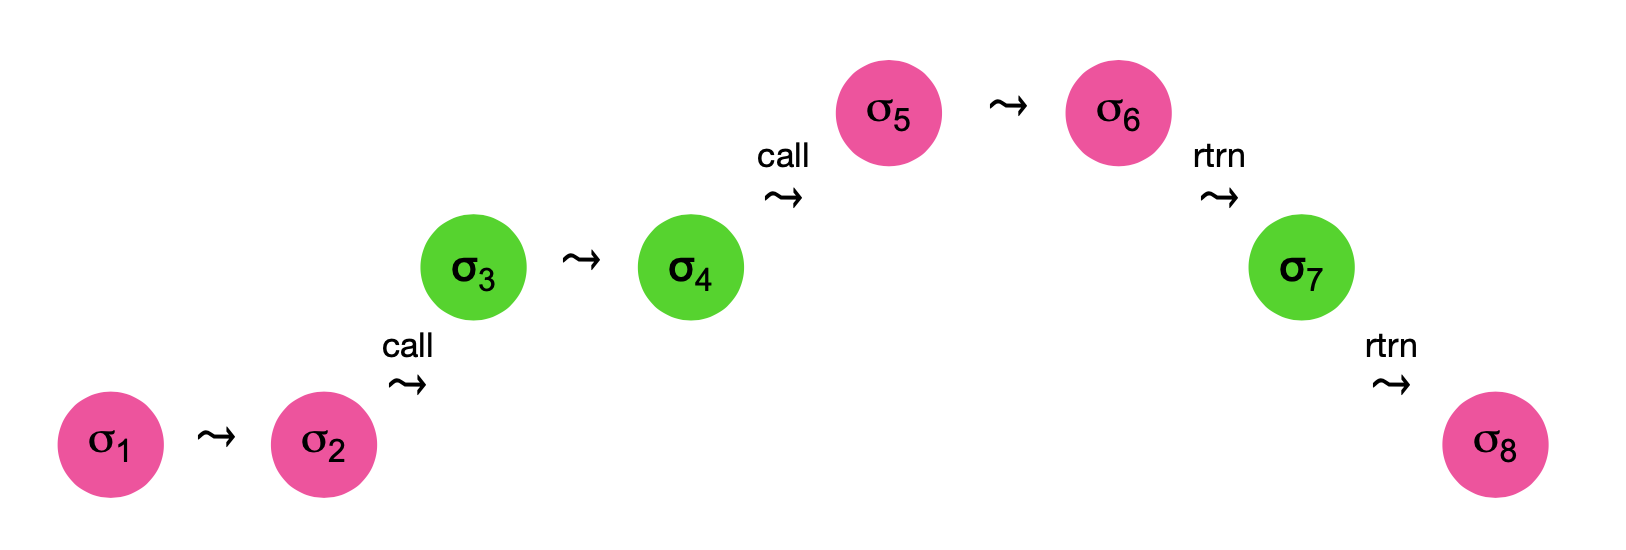
\includegraphics[width=\linewidth]{diagrams/ObservableStates1.png}
} 
&
\resizebox{6.5cm}{!}{
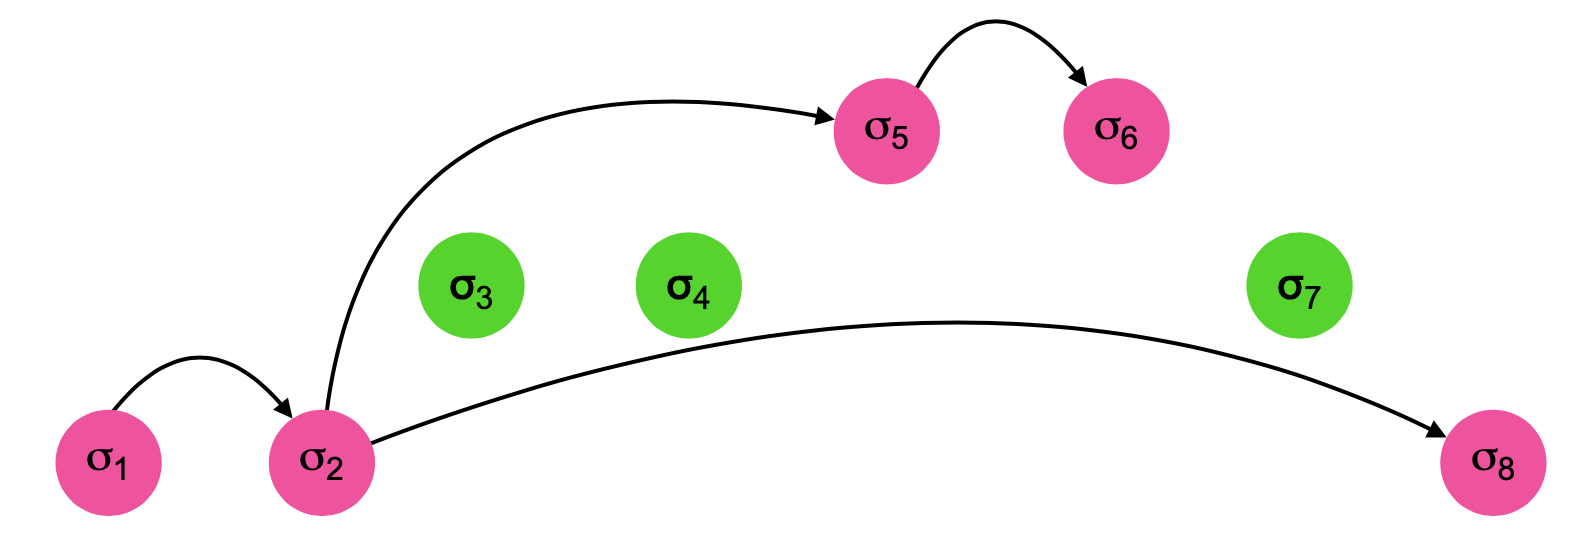
\includegraphics[width=\linewidth]{diagrams/ObservableStates2.png}
}
\\
\hline
\\
$\exec{{\color{hotpink}M_{ext}} \circ {\color{lightseagreen}M}}{{\color{hotpink}\sigma_1}} {{\color{hotpink}\sigma_2}}
 \leadsto {{\color{lightseagreen}\sigma_3}}  \leadsto {{\color{lightseagreen}\sigma_4}}
\leadsto {{\color{hotpink}\sigma_5}} $
&
$\reduction{{\color{hotpink}M_{ext}}}{{\color{lightseagreen}M}}{{\color{hotpink}\sigma_1}} {{\color{hotpink}\sigma_2}}
 \redsymb   {{\color{hotpink}\sigma_5}} \redsymb   {{\color{hotpink}\sigma_6}}$
\\
$\exec{{\color{hotpink}M_{ext}} \circ {\color{lightseagreen}M}}{{\color{hotpink}\sigma_5}} {{\color{hotpink}\sigma_6}}
\leadsto{ {\color{lightseagreen}\sigma_7}}
\leadsto {{\color{hotpink}\sigma_8}}$ &
$\reduction{{\color{hotpink}M_{ext}}}{{\color{lightseagreen}M}}{{\color{hotpink}\sigma_2}} {{\color{hotpink}\sigma_8}}$
\\
\hline
\end{tabular}
   \caption{Illustrating Observable States Semantics
     (Def. \ref{def:pair-reduce}) %
    }
   \label{fig:VisibleStates}
 \end{figure}
 
Fig. \ref{fig:VisibleStates} % inspired by \citeasnoun{FASE}
 provides a simple graphical description of 
our {observable} states semantics: on the left hand side is the ``normal'' execution after 
linking two modules into one: \ ${\color{hotpink}M_{ext}} \circ {\color{lightseagreen}M}, ... \leadsto ...$. We assume  that
the receiver in states ${\color{hotpink}\sigma_1}$, ${\color{hotpink}\sigma_2}$, ${\color{hotpink}\sigma_5}$, ${\color{hotpink}\sigma_6}$, and ${\color{hotpink}\sigma_8}$ is from ${\color{hotpink}M_{ext}}$, and that 
 the receiver in ${\color{lightseagreen}\sigma_3}$, ${\color{lightseagreen}\sigma_4}$ and ${\color{lightseagreen}\sigma_7}$ is from ${\color{lightseagreen}M}$.
 Moreover, we assume that the transition from ${\color{hotpink}\sigma_2}$ to ${\color{lightseagreen}\sigma_3}$ corresponds to a call of an internal method, and the transition from ${\color{lightseagreen}\sigma_4}$ to ${\color{hotpink}\sigma_5}$ corresponds to  a call of an external method. We also assume that the transition from ${\color{hotpink}\sigma_6}$ to ${\color{lightseagreen}\sigma_7}$ corresponds to the termination of the latter, while the transition from ${\color{lightseagreen}\sigma_7}$ to ${\color{hotpink}\sigma_8}$ corresponds to the termination of the former.
The right hand side illustrates the 
observable states execution. Note that the $redsymb$ relation only holds between {\color{hotpink}external} states. Note also that
while $\exec{{\color{hotpink}M_{ext}} \circ {\color{lightseagreen}M}} {\color{hotpink}\sigma_6} {\color{lightseagreen}\sigma_7} \leadsto {\color{hotpink}\sigma_8}$, there is no $\redsymb$ relation between ${\color{hotpink}\sigma_6}$ and ${\color{hotpink}\sigma_8}$. 

 %\footnote{Note that whether a module is external or internal depends on %our
%perspective -- nothing in a module itself renders it internal or external. For example, in
% $\reduction{M_1}{M_2}{...}{...}$ the external module is $M_1$,
%  while in  $\reduction{M_2}{M_1}{...}{...}$  the external module is $M_2$.
%}
\footnote{{TODO: say how observable states differs from visible states, and from OOPLSA external states.}}

We  use the notation\ \  $\reductions{M_{ext}}{M}{\sigma}{\sigma'}$ \ 
to denote zero or more  steps starting at state $\sigma$ and ending at state $\sigma'$, in the context of internal module 
$M$ and external module $M_{ext}$.
 Note that $\redsymb^*$ is --obviously-- transitive.
 
 %Not only are we unconcerned 
%with internal states,  we are also unconcerned with  states which cannot ever arise from execution.
We are {not} concerned with internal states or states that can never arise.
{A state $\sigma$ is \emph{arising},}  written $\arising{\sigma}{M_{ext}}{M}$, {if it  may arise by observable states} execution
starting at some initial configuration:

\subsubsection{Arising States}

\begin{definition}[Arising  States]
\label{def:arising}
For   modules $M$ and  $M_{ext}$, a % program
 state $\sigma$ is 
called an \emph{arising} state, formally \ \ \ $\arising{\sigma}{M_{ext}}{M}$,\ \ \ 
if and only if there exists some $\sigma_0$ such that $\initial{\sigma_0}$ and
$\reductions{M_{ext}}{M}{\sigma_0}{\sigma}$.
\end{definition}


An \emph{Initial} state's heap contains a single object of class \prg{Object}, and
its  stack   consists of a single frame, whose local variable map is a
mapping from \prg{this} to the single object, and whose continuation is  any statement.
(See Definition %s \ref{def:initial} and 
\ref{def:arising} and the 
{appendices %of the full paper 
\cite{necessityFull}).}

$ \arising{\sigma}{M_{ext}}{M}$, implies that $\sigma$ is an external state, since  $M_{ext} \circ M, \sigma  \leadsto^* \sigma' $ implies that both $\sigma$ and $\sigma'$ are external states.


\subsubsection{{Reachable  Objects}}

\footnote{{TODO: this logically belongs here,  but how to motivate? -- Perhaps something will have been said in the intro?}}


We adopt notation from OOPSLA, where
 $\interpret{\phi}{x} = v$  means that $x$ maps to
value $v$ in the local variable map of frame $\phi$, $\interpret{\sigma}{x} = v$ means that $x$ 
maps to $v$ in the top most frame of $\sigma$'s stack, and $\interpret{\sigma}{x.f} = v$
has the obvious meaning. The terms $\sigma.\prg{stack}$,  
$\sigma.\prg{contn}$,  
$\sigma.\prg{heap}$     mean the stack, 
the continuation at the
top frame of $\sigma$, %resp. 
and the heap of $\sigma$.
The term $\alpha\!\in\!\sigma.\prg{heap}$ means that $\alpha$ is in the domain of the heap of $\sigma$, and \emph{$x$ fresh in $\sigma$} means that 
$x$ isn't in the variable map of the top frame of $\sigma$, 
while the substitution  $\sigma[x \mapsto \alpha]$ is applied to the top frame of $\sigma$.
 \ $C\in M$ means that class $C$ is in the domain of module $M$. 


\subsubsection{{Reachable  Objects and Observable States}}


The lemma below is the counterpart to lemma \ref{lemma:relevant}:

\begin{lemma}
For all $\sigma$, $\sigma'$, for all objects $o$, and for all modules $M_{ext}$, and $M$:
\begin{itemize}
\item
$\reduction {M_{ext}} {M} {\sigma} {\sigma'} \ \wedge \  \GRelevant o {\sigma'} \ \wedge \ o\in dom(\sigma) \ \ \Longrightarrow \ \  \GRelevant o {\sigma}$.
\item
$\reduction {M_{ext}} {M} {\sigma} {\sigma'} \ \wedge \    \LRelevant o {\sigma'}\   \wedge \ o\in dom(\sigma) \ \ \Longrightarrow \ \  \LRelevant o {\sigma}$.
\end{itemize}
\end{lemma}

\subsection{Semantics of Assertions}

We now give meaning to assertions. Definitions (1)-(5) are standard. Note that Definitions (6)-(7) quantify only over objects that are accessible from the top frame. TODO  explain that the sequence of field reads $\prg{f}_1$,.....$\prg{f}_n$ may be empty,
An illustration of the concept of reachable appears in the next subsection, in Fig. \ref{fig:Relevant}.

 

\subsection{\AssertLang -- the assertion language}
\label{sub:SpecO}

Our assertions language, \AssertLang, extends a 
 basic assertion language extended with
object-capability assertions. 


\subsubsection{Syntax of \AssertLang}
The syntax of \AssertLang   is given in
Definition \ref{f:chainmail-syntax}.
An assertion may be an expression,   a query of the defining class of
  an object, the usual connectives and quantifiers, along 
with two non-standard assertion forms:
(1) \emph{Internal/external} and (2) \emph{Protection}, inspired by the capabilities literature, and
\footnote{{ TODO say how these relate with capability lit;  compare with 
 OOPSLA.}}


\begin{definition}
Assertions ($A$) in
\AssertLang are defined as follows:

\label{f:chainmail-syntax}
 \[
\begin{syntax}
\syntaxElement{A}{}
		{
		\syntaxline
				{{\re}}
				{{\re} : C}
				{\neg A}
				{A\ \wedge\ A}
				{A\ \vee\ A}
				{\all{x:C}{A}}
				{\ex{x:C}{A}}
		\endsyntaxline
		}
		{
		\syntaxline
				{\internal{{\re}}}
				{\protectedFrom{{\re}} {{\re}}} 
				 {\inside {{\re}}} 
		\endsyntaxline
		}
\endSyntaxElement\\
\end{syntax}
\]

\sdOct{\textbf{NOTE}  This allows for the ugliness that we can write assertions like $\alpha.bal > 700$ which obviously makes no sense without a $\sigma$. We could say that assertion that contain variables are the run-time counterpart of those which do not. Also, note that universal quantification over expressions ($\forall \alpha:C.[A]$) is not supported\footnote{This may only be a techncality, though}. On the other hand, $a.bal > 700$ does not make sense without a $\sigma$ either.
}

\sdOct{\textbf{NOTE} It also allows assertions like $a1.passwd \neq a2.passwd$, whereas in the past we would have written as
$\exists x,y.[\ a1.passwd=x \wedge  a2.passwd=y \wedge x\neq y\ ]$.}


\end{definition}

\footnote{{TODO compare with oopsla }}


\subsubsection{Semantics of \AssertLang}
The semantics of \AssertLang   
is given in Definition \ref{def:chainmail-semantics}. 
We   use the evaluation relation, $\eval{M}{\sigma}{e}{v}$,
which says that the expression $e$ evaluates
to value $v$ in the context of state $\sigma$ and module $M$.
As expressions in \LangOO may be recursively defined, their evaluation 
need not   % may not necessarily 
 terminate. Nevertheless, the logic of $A$ remains classical because recursion is restricted
to expressions, and not generally to assertions.
\footnote{We have taken this approach from \citeasnoun{FASE}, which also contains a mechanized Coq proof that assertions are classical \cite{coqFASE}.
%  The full
The semantics of $\hookrightarrow$ {is} unsurprising 
(see {the appendices %of the full paper 
\cite{necessityFull}).} } %Fig.\ref{f:evaluation}).



begin{definition}[Satisfaction 
of Assertions by a module and a state] 
\label{def:chainmail-semantics}
We define satisfaction of an assertion $A$ by a % program 
state $\sigma$ with 
 module $M$ as:
\begin{enumerate}
\item
\label{cExpr}
$\satisfiesA{M}{\sigma}{\sdOct{\re}}$ \ \ \ iff \ \ \  $\eval{M}{\sigma}{\sdOct{\re}}{\true}$
\item
\label{cClass}
$\satisfiesA{M}{\sigma}{{\sdOct{\re}} : C}$ \ \ \ iff \ \ \  $\eval{M}{\sigma}{\sdOct{\re}}{\alpha}\   \wedge \ \class{\alpha} {\sigma}= C$
\item
$\satisfiesA{M}{\sigma}{\neg A}$ \ \ \ iff \ \ \  ${M},{\sigma}\nvDash{A}$
\item
$\satisfiesA{M}{\sigma}{A_1\ \wedge\ A_2}$ \ \ \ iff \ \ \  $\satisfiesA{M}{\sigma}{A_1} \   \wedge \ \satisfiesA{M}{\sigma}{A_2}$
\item
$\satisfiesA{M}{\sigma}{A_1\ \vee\ A_2}$ \ \ \ iff \ \ \  $\satisfiesA{M}{\sigma}{A_1}\   \vee \ \satisfiesA{M}{\sigma}{A_2}$

\item
\label{quant1}
$\satisfiesA{M}{\sigma}{\all{x:C}{A}}$ \ \ \ iff \ \ \  
 \sdOct{$\forall \alpha.[\ \GRelevant \alpha \sigma \wedge  \satisfiesA {M}{\sigma} {\alpha:C}  \ \Longrightarrow   \ \satisfiesA{M}{\sigma} {A[x/\alpha]}\ ]$.} 
% $\satisfiesA{M}{\sigma[x \mapsto o]}{x:C} \ \ \Longrightarrow \ \ \ \satisfiesA{M}{\sigma[x \mapsto o]}{A}$, \\
%\strut \hspace{1.3in}  \sd{for all  $o$ such that $ \GRelevant o \sigma$ }%, where $x$ is free in $\sigma$ } 

\item
\label{quant2}
$\satisfiesA{M}{\sigma}{\ex{x:C}{A}}$ \ \ \ iff \ \ \  
 \sdOct{$\exists \alpha.[\ \GRelevant \alpha \sigma \wedge  \satisfiesA {M}{\sigma} {\alpha:C}  \ \wedge \ \satisfiesA{M}{\sigma} {A[x/\alpha]}\ ]$.} 
% $\satisfiesA{M}{\sigma[x \mapsto o]}{x:C} \ \ \wedge \ \ \ \satisfiesA{M}{\sigma[x \mapsto o]}{A}$, \\
%\strut \hspace{1.3in}  \sd{for some $o$ such that $\GRelevant o \sigma$. } %, where $x$ is free in $\sigma$. }
\item
\label{cInternal}
$\satisfiesA{M}{\sigma}{\internal{\sdOct{\re}}}$ \ \ \ iff \ \ \   $\satisfiesA{M}{\sigma}{{\sdOct{\re}} : C} \ \wedge\ \ C \in M$
\item
\label{cExternal}
$\satisfiesA{M}{\sigma}{\external{\sdOct{\re}}}$ \ \ \ iff \ \ \   $\satisfiesA{M}{\sigma}{{\sdOct{\re}} : C} \ \wedge \ C \notin M$
\item
\label{cProtected}
$\satisfiesA{M}{\sigma}{\protectedFrom{\sdOct{\re}} {\sdOct{\re_{o}}}}$  \ \ \ iff \\
  $\exists \alpha, \alpha_{o}. [\ $
\begin{enumerate}
\item $\eval{M}{\sigma}{\sdOct{\re}}{\alpha} \ \ \ \wedge\ \ \  \eval{M}{\sigma}{\sdOct{\re_{o}}}{\alpha_{o}}$, \ \ \ \ \ \ and  
\item
\sdOct{$\alpha \neq \alpha_{o}$}, % \footnote{!!!! \  NOT THAT SURE HERE, but think so !}
\ \  \ \ \  and 
\item 
\sdOct{$\forall n\in\mathbb{N}. \forall f_1,...f_n.$\\
$
%\strut \hspace{1cm} 
[\ \ \interpret{\sigma}{\alpha_{o}.f_1...f_n}=\alpha \ \wedge\ \forall k\!<\!n.\interpret{\sigma}{\alpha_{o}.f_1...f_k}\neq \alpha \ \
% $\\ $ \strut \hspace{5.5cm} \   
\ \  \Longrightarrow \ \ \satisfiesA{M} {\sigma} {\internal{{\alpha_{o}.f_1...f_{n-1}}}}\ \ ]$}
\end{enumerate}
\strut \hspace{.4cm} $]$
% The previous version 
%\begin{enumerate}
%\item $\satisfiesA{M}{\sigma}{x \neq z}$  and
%\item
%$\forall f_1,...f_n.[\ \interpret{\sigma}{z.f_1...f_n}=\interpret{\sigma}{x} \ \Longrightarrow \exists k<n.
%[\,\satisfiesA{M}{\sigma}{\internal{z.f_1...f_k}} \, ] \ ]$ and
%\item either
%\begin{enumerate}
%\item $\satisfiesA{M}{\sigma}{z \neq \this}$ or
%\item $\forall y.[y \in \sigma.\texttt{local}
%\Longrightarrow \satisfiesA{M}{\sigma}{(\internal{y} \wedge y \neq x) \vee \protectedFrom{x}{y}}]$
%\end{enumerate}
%\end{enumerate}
\item
$\satisfiesA{M}{\sigma} {\inside {\re}}$   \ \ \ iff \ \ \  
\sdOct{$\forall \alpha.[ \  \LRelevant {\alpha}  {\sigma}\ \Longrightarrow \ \  \satisfiesA{M}{\sigma}{\protectedFrom{\re} {\sdOct{\alpha}}}\ ] $}
\end{enumerate}
%\end{definition}

Say that $\Longrightarrow$ is meta, while $\rightarrow$ is Chainmail.
\footnote{{TODO: explain that$x$ is fresh in $\sigma$  means that $x$ is not in the domain of the top frame, nor in the top continuation of $\sigma$.
 Note, the assumption $x$ is fresh in $\sigma$ has to be justified. Barendregt convention? Or say how we rename if $x$ is not free.}}

{Both existential and universal quantification (defined in \ref{quant1} and \ref{quant2}) is done over all objects which are transitively 
accessible any frame in the stack (as in OOPSLA). But note that $\satisfiesA{M}{\sigma} {\inside {y}}$ only considers objects that are locally relevant.
We do not include quantification over primitive types such as integers as \LangOO is too simple. The 
Coq mechanisation does include primitive types.}
 
\footnote{{TODO: say that any assertion $A(e)$ can be understood as a shorthand for $\exists x. [ x=e \wedge A(x)]$. or  $forall x. [ x=e \rightarrow A(x)]$?? For example, the  assertion   ${\internal{e}}$ is a shorthand for $\exists x. [ x=e \wedge {\internal{x}}]$. QUESTION: do we need to talk about $=$ in the assertion language?}}

 Note that in most cases, satisfaction of an assertion not only depends on the state $\sigma$, but 
in some cases it also depends on the module: namely execution of expressions (\ref{cExpr}) might need to look up the definition of ghost fields  in $M$, while 
for internal or external provenance (\ref{cInternal} and \ref{cExternal}) we need to know all the classes defined in $M$.


${\inside {\_}}$  is central to thiking about capabilities. For example, the balance of an account whose
  password is  encapsulated/protected?  will not decrease in the next step.
  Often, API implementations contain objects whose capabilities, while  crucial for the implementation, if exposed,
would break the intended guarantees of the API. Such objects need to remain confined - see
such an example in Section \ref{s:examples}. 

\sdOct{\textbf{NOTE} in the def of  $\protectedFrom{\re}{\re_o}$, when enumerate the paths that go from $\re_o$ to $\re$, we exclude those that have already "visited" $\re$ earlier on. That is, we only consider the direct paths from $\re_o$ to $\re$. This is pretty much what "dominates" means- James you were right -- put it is a "relative" domination}

\sdOct{\textbf{NOTE} also, that the term $\re$ may mention ghost fields, but the paths $\alpha.f_1....f_n$ may not. We see that because the latter are interpreted in $\sigma$. That is, $\satisfiesA{M}{\sigma}{\sdOct{\alpha_o.f_1...f_n}=\alpha}$ is weaker than $\interpret{\sigma}{\alpha_{o}.f_1...f_n}=\alpha$. TODO: write the latter as a lemma}

\sdOct{\textbf{NOTE} to reflect a bit more on (10)(b) from above}
 
\footnote{{. TODO: Do we prove the implications as in TACAS, or just rely on TACAS? -- perhaps the former, since we have some new primitives? hmhh}}

\begin{figure}[htb]
\begin{tabular}{|c|c|c|}
\hline \\
\resizebox{4.5cm}{!}{
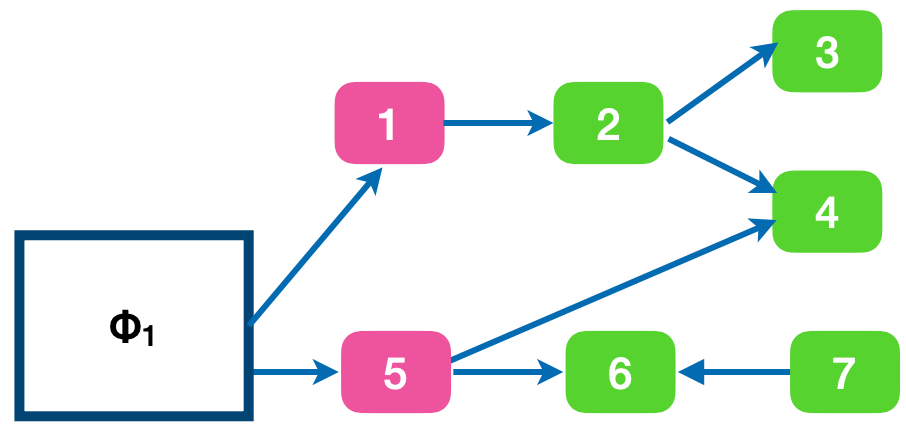
\includegraphics[width=\linewidth]{diagrams/prot1.png}
} 
&
\resizebox{4.5cm}{!}{
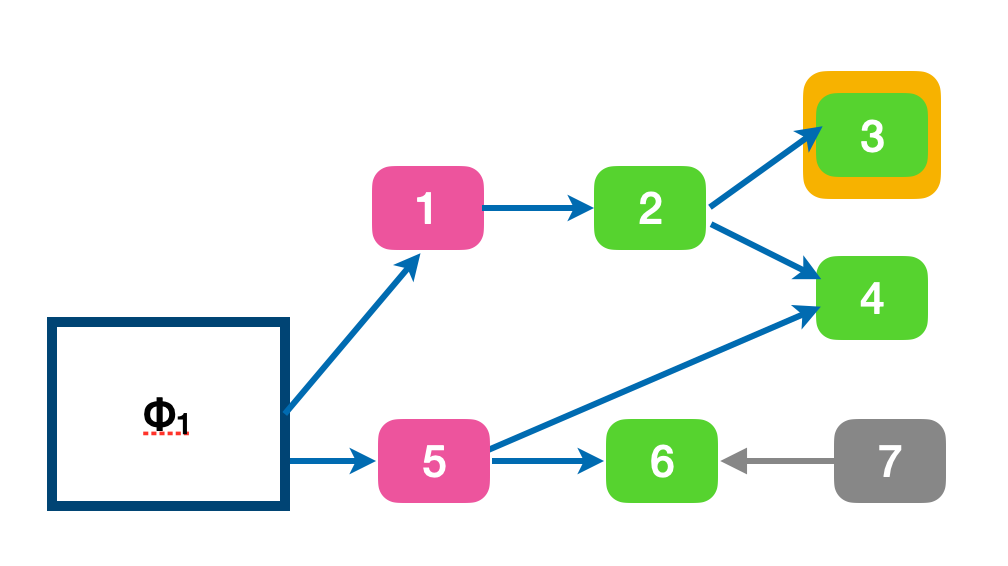
\includegraphics[width=\linewidth]{diagrams/prot2.png}
} 
&
\resizebox{4.5cm}{!}{
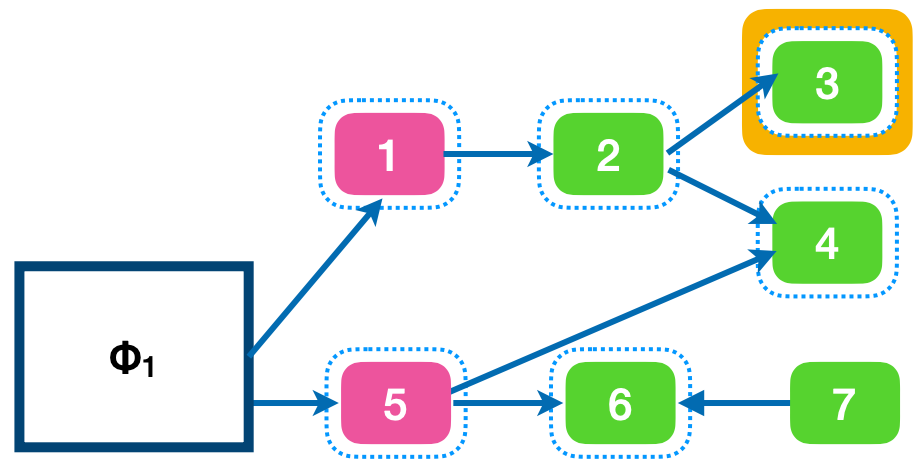
\includegraphics[width=\linewidth]{diagrams/prot3.png}
} 
\\
\hline
 $\sigma_1$ 
&
Locally Relevant: $1$, $2$, $3$, $4$,  $5$,  $6$. 
&
Protected: $3$
\\
\hline \hline
 \\
\resizebox{4cm}{!}{
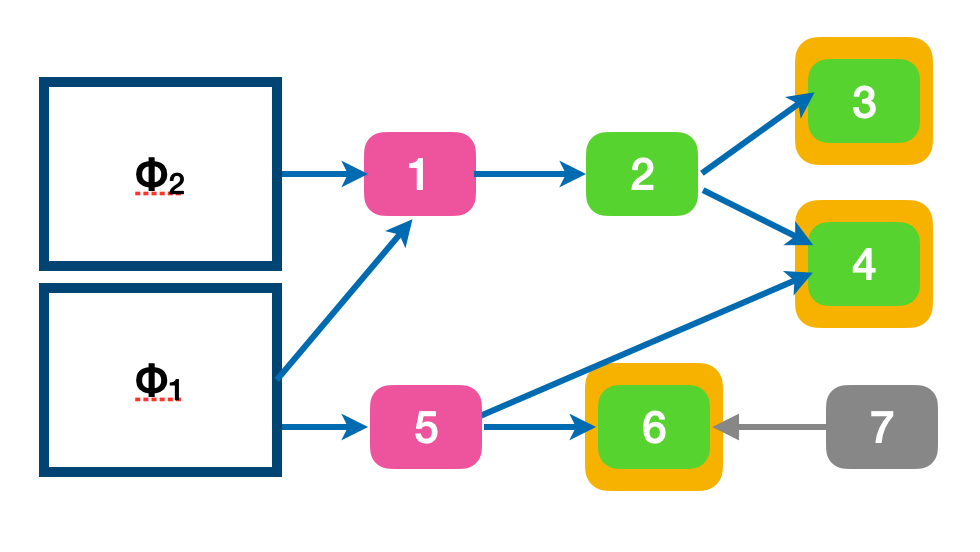
\includegraphics[width=\linewidth]{diagrams/prot4.png}
} 
&
\resizebox{4cm}{!}{
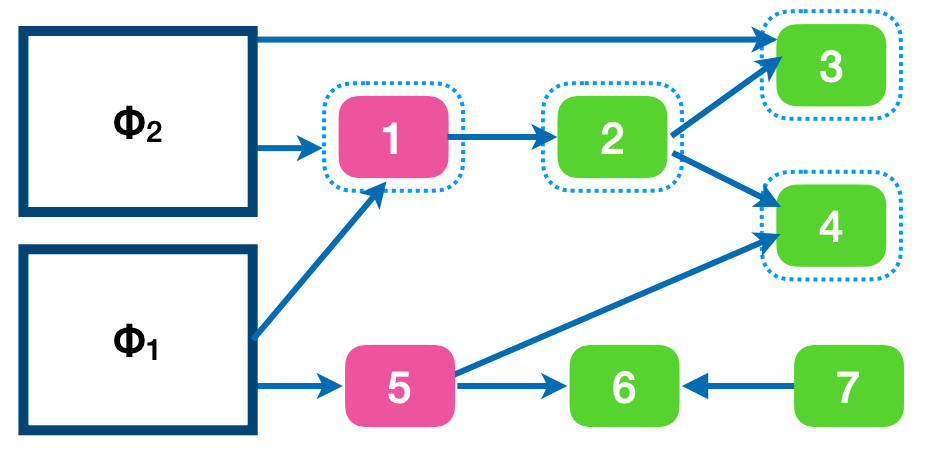
\includegraphics[width=\linewidth]{diagrams/prot5.png}
} 
&
\resizebox{4cm}{!}{
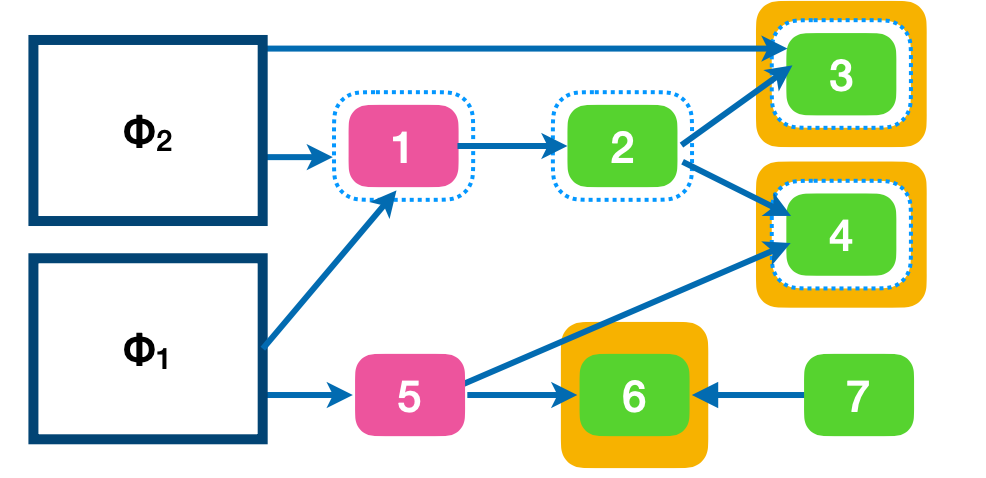
\includegraphics[width=\linewidth]{diagrams/prot6.png}
} 
\\
\hline
 $\sigma_2$ 
&
Locally Relevant: $1$, $2$, $3$, $4$.
& 
Protected: $3$, $4$, $6$
 \\
\hline \hline
\end{tabular}
   \caption{Relevant Objects and Protection. Square boxes are frames ($\phi_1$ and $\phi_2$).   Rounded boxes are objects;  external objects in pink (here $1$ and $5$);   internal objects in green (here $2$, $3$,  $4$, $6$ and $7$). 
   Locally relevant objects indicated through the dotted blue outline,  and protected objects have a golden background. \\
 }
   \label{fig:Relevant}
 \end{figure}
 
 
Figure \ref{fig:Relevant} illustrates the concepts of relevant and protected. On the first line, the   three diagrams illustrate $\sigma_1$, a state with one frame on the stack ($\phi_1$), and   a heap with 7 objects. 
The second line depicts the next  state, $\sigma_2$, where we just made a method call: we have the same heap, and have pushed a fresh frame, $\phi_2$,  on the stack.

Relative protection does not depend on the frames, and therefore is identical in the two states. We therefore have:\\
~ \strut \hspace{.2cm}  
$\satisfiesA{M}{\sigma_1}{\protectedFrom{3} {1}}$, \ \  \ \ 
$\satisfiesA{M}{\sigma_1}{\protectedFrom{4} {1}}$, \ \  \ \ 
$M, \sigma_1 \not\models {\protectedFrom{4} {5}}$.\\
~ \strut  ~ \hspace{.2cm}  
$\satisfiesA{M}{\sigma_2}{\protectedFrom{3} {1}}$, \ \ \ \ 
$\satisfiesA{M}{\sigma_2}{\protectedFrom{4} {1}}$, \ \  \ \ 
$M, \sigma_2 \not\models {\protectedFrom{4} {5}}$.\\
On the other hand, Local relevance does depend on the frames, and so we have:
\\
~ \strut \hspace{.2cm}  
$ \LRelevant{ \{\,1, 2, 3, 4, 5, 6\, \}}{\sigma_1}$, \ \  \ \ $\neg {\LRelevant { \,7\, }  {\sigma_1}}$.\\
~ \strut  ~ \hspace{.2cm}  
$\LRelevant{ \{\, 2, 3, 4\,  \} }{\sigma_2}$, \ \  \ \ $\neg {\LRelevant{ \{\, 5, 6, 7\,  \} } {\sigma_2}}$. \\
Therefore, protection in the two states is as follows:\\
~ \strut \hspace{.2cm}  
$\satisfiesA{M}{\sigma_1}{\inside{\, 3 \, }}$, \ \  \ \   $M, \sigma_1 \not\models {\inside{ \, \{1, 2, 4, 5, 6, 7\} \, }}$.\\
~ \strut \hspace{.2cm}
$\satisfiesA{M}{\sigma_2}{\inside{\, \{\, 3, 4, 6\, \}  \, }}$, \ \  \ \   $M, \sigma_2 \not\models {\inside{ \, \}1, 2, 5, 7\} \, }}$.
 

\subsection{\SpecLang specifications}


\noindent
The syntax of  \SpecLang specifications is given below
 
\begin{definition}  

\noindent
{\emph{{Syntax of \SpecLang Specifications}}}

\label{f:holistic-syntax}
\[
\begin{syntax}
\syntaxElement{S}{}
		  {\syntaxline
                               {\OneStateQ {\overline {x:C}} {A} }	
				{\TwoStatesQ {\overline {x:C}} {A} {A} }	
				{S\, \wedge \, S}
		 \endsyntaxline
		}
\endSyntaxElement\\
\end{syntax}
\]
\end{definition}

\label{sec:adapt:motivate}




\subsubsection{ Semantics of \SpecLang Specifications}
We now  define what it means for  a module  $M$ to satisfy specification  $S$, written as $M \vDash S$. The
 
\begin{definition}% [Semantics of \SpecLang Specifications]

We define $\satisfies{M}{{S}}$ by cases over the four possible syntactic forms.
For any assertions   $A_1$, $A_2$, and $A$: \\

\label{def:necessity-semantics}

\begin{tabular}{l l c l }

$\bullet$ & $\satisfies{M}{\OneStateQ {\overline {x:C}} {A} 	}$& iff & 
for all $M_{ext}$, $\sigma$, $\overline{x}$, such that $\overline{x}$  are free in $\sigma$, \\
  & & & $ \arising{\sigma}{M_{ext}}{M}$ % \ \wedge 
$ \ \Longrightarrow \  $  % \\ & & &  $ \satisfiesA{M}{\sigma[\overline{x\mapsto o}]}{A} $
{$ \satisfiesA{M}{\sigma}{\forall \overline{x:C}.A}$}\footnote{{This means that we require all objects to satisfy even if not locally relevant}}
\\
\\
$\bullet$ & $\satisfies{M}{\TwoStatesQ {\overline {x:C}} {A}{A'}}$& iff & 
for all $M_{ext}$, $\sigma$, $\overline{x}$, $\overline{o}$ such that $\overline{x}$  are free in $\sigma$  \\
& & &
$\arising{\sigma}{M_{ext}}{M} \ \wedge\  \GRelevant {\overline o}  \sigma \wedge \ $\footnote{{notice that we are asking for globally relevant objects}}\\
& & & $ \satisfiesA{M}{\sigma[\overline{x\mapsto o}]}{\overline {x:C}}  \ \ \wedge\ \  \satisfiesA{M}{\sigma[\overline{x\mapsto o}]}{A} \ \ \wedge$ \\ 
& & &
$\reductions{M_{ext}}{M}{\sigma}{\sigma'}  $ \\
& & & $ \Longrightarrow $ \\
& & & $ \satisfiesA{M}{\sigma'[\overline{x\mapsto o}]}{A'} $
\\
\\
$\bullet$ &  $\satisfies{M}{S\, \wedge\, S'}$ &   iff   & $\satisfies{M}{S}\ \wedge \ \satisfies{M}{S'}$
\end{tabular} 

 
\end{definition} 

  
  \footnote{{TODO: Make an example that demonstrates the difference if in the second bullet we had asked for locally relevant objects ${\overline o}$.}}
 
\footnote{{TODO Notice that we assume that $\overline x$ are not free in $A$ -- cf Barendregt convention.}}




And try this first $\TwoStatesQ {\prg{a}:\prg{Account}}  {\inside{\prg{a.password}}} {\inside{\prg{a.password}}}$

\subsection{Specification Examples}
\noindent
As an example, consider the following    specifications:

\begin{tabular}{lcll}
$S_1$   &     $\triangleq$   & $\OneStateQ{\prg{a}:\prg{Account} } {\inside{\prg{a}}} $
 \\
 $S_2$   &     $\triangleq$   & $\OneStateQ{\prg{a}:\prg{Account} } {\inside{\prg{a.password}}} $
 \\
 $S_3$   & $\triangleq$   &  $\TwoStatesQ {\prg{a}:\prg{Account}}  {\inside{\prg{a}}} {\inside{\prg{a}}} $
 \\
 $S_4$   & $\triangleq$   &  $\TwoStatesQ {\prg{a}:\prg{Account}}  {\inside{\prg{a.password}}} {\inside{\prg{a.password}}}$
 \\
$S_5$ & $\triangleq$   &
 $\forall \prg{a}:\prg{Account}.\forall \prg{b}:\prg{int}.$\\
  &  &  $\FirstState{\inside{\prg{a}} \wedge \prg{a.balance}=\prg{b}} 
\  \SecondState{ \prg{a.balance}= \prg{b} }$
\\
$S_6$ & $\triangleq$   &
  $\forall \prg{a}:\prg{Account}.\forall \prg{b}:\prg{int}.$\\
  &  &  $\FirstState{\inside{\prg{a.password}} \wedge \prg{a.balance}=\prg{b}} 
\  \SecondState{ \prg{a.balance}\geq \prg{b} }$
 \end{tabular}

\vspace{.2cm}
Now consider our modules from earlier. We have that

\begin{tabular}{lllllll}
$\ModA \not\models S_1$  & & $\ModA \not\models S_2$ &&  $\ModB \not\models S_1$ &  &$\ModB \not\models S_2$ \\
$\ModA \models S_3$ & &   $\ModA \models S_4$ & &  $\ModB  \models S_3$ & &  $\ModB  \not\models S_4$ \\
$\ModA \models S_5$ & &  $\ModA \models S_6$ & & $\ModB  \models S_5$ & & $\ModB   \not\models S_6$ \\
\end{tabular}

\vspace{.6cm}
Consider also  $S_{4a}$ which is a variation of $S_4$, as well as $S_7$, which ...

\begin{tabular}{lcll}
$S_{4a}$   &     $\triangleq$   &   ${\TwoStatesQ {\prg{a}:\prg{Account}.\prg{p}:\prg{Password}}  {\prg{p}=\prg{a.password} \wedge \inside{\prg{p}}}{\inside{\prg{p}}} }$
 \\
$S_7$ & $\triangleq$   & ${\TwoStatesQ {\prg{a}:\prg{Account}.\prg{p}:\prg{Password}}  {\prg{p}=\prg{a.password}} {\prg{p}=\prg{a.password}} }$
 \end{tabular}
 
 \noindent
 Fort these specifications
 
 \begin{tabular}{lllllll}
$\ModA  \models S_7$  & & $\ModB \not\models S_7$ &&  $\ModC \not\models S_7$ \\
\end{tabular}

\subsection{Tautological assertions, and Specification Implication}

\begin{definition}[Satisfaction of Assertions by a module] 
\label{def:assertion-inference-semantics}
We define satisfaction of an assertion $A$ by a  module $M$ as:
\begin{itemize}
\item
$M \vDash A$   \ \ \ iff \ \ \  $\forall M_{ext}. \forall \sigma.[\ \arising{\sigma}{M_{ext}}{M} \ \Longrightarrow \ \ \satisfiesA{M}{\sigma}{e}\ \ ]$
\end{itemize}
\end{definition}

TODO: Here we will say that assertions are classical, as proven in FASE

\begin{definition}[Stronger Specifications] 
\label{def:specification-implication-semantics}
We define when a specification $S$ is stronger than another specification $S'$  in the context of a  module: 
 \begin{itemize}[itemsep=5pt]
\item 
$\stronger M  S  {S'}$   \ \ \ iff \ \ \  $M\models S$ implies $M \models S'$
\item
$\strongerEq M  S  {S'}$   \ \ \ iff \ \ \ $\stronger M  S  {S'}$  \ and \  $\stronger M   {S'} S$    
\end{itemize}
\end{definition}

We know about stronger specifications:

\begin{lemma}
Consider assertions $A$, $A'$, variable $y$ free in $A$, specifications $S$, $S'$, and module $M$:
\begin{itemize} [topsep=6pt,itemsep=5pt,parsep=0pt,partopsep=0pt]
\item
$\stronger M {\OneStateQ {\overline {x:C}}  {A}}  {\TwoStatesQ {\overline {x:C}} {A}{A}} $ 
    \item
 $\strongerEq  M  {\OneStateQ    {y:\prg{Object}}   {\forall \overline {x:C}[ A ] } } 
    {\OneStateQ {\overline {x:C}}  {A}} $.
\item
$  M  \models (  \overline {x:C} \wedge A) \rightarrow A'$ \ \ \  implies \ \  \ $\stronger M  {\OneStateQ {\overline {x:C}} {A}}    {\OneStateQ {\overline {x:C}} {A'}}$
\item
  \ $\stronger M  { \TwoStatesQ {y:\prg{Object}}  {\forall x:C.[A]} {\forall x:C.[A']} }    {\TwoStatesQ {\overline {x:C}} {A}{A'}} $

\item
$\stronger M  S {S''}$ and $\stronger M {S''} {S'}$\ \  implies \ \ $\stronger M S  {S'}$.
\end{itemize}

\end{lemma}



